%FOR PDFLATEX USE ONLY
\documentclass[a4paper,12pt]{article}

\usepackage{amssymb,amsmath}

\usepackage[margin=2cm]{geometry}
\usepackage[unicode]{hyperref}
\usepackage[pdftex]{graphicx}
\usepackage{cmlgc}

\usepackage{array}

\usepackage{wrapfig}
\usepackage{array}
\usepackage{lipsum}
\usepackage{esvect}
\usepackage{hyperref}

\usepackage{subfig}
\usepackage{calc}
\usepackage{pgfplots,tikz,circuitikz}
\usepackage{pgfplotstable}
\usepackage{tkz-euclide}

\usepackage{centernot}
\usepackage{cancel}

\usepackage{mathtext}
\usepackage[T1,T2a]{fontenc}
\usepackage[utf8]{inputenc}
\usepackage[english, bulgarian, russian]{babel}
\usepackage{tikz}
\usepackage{pgfplots}
\usepackage[export]{adjustbox}
\usepackage[left=2cm,right=2cm,
    top=2cm,bottom=2cm,bindingoffset=0cm]{geometry}
\usepackage{indentfirst}
\usepackage{braket}

\begin{document}

\begin{center}
  \LARGE{Работа 2.2.3}\\[0.2cm]
  \LARGE{ИЗМЕРЕНИЕ ТЕПЛОПРОВОДНОСТИВОЗДУХА ПРИ АТМОСФЕРНОМ ДАВЛЕНИИ}\\[0.2cm]
  \large{Панферов Андрей}\\[0.2cm]
\end{center}

\textbf{Цель работы:} измерить коэффициенттеплоп  роводности воздуха при атмосферном давлении в зависимости от температуры. 

\textbf{В работе используются:} цилиндрическая колба с натянутой по оси нитью; термостат; вольтметр и амперметр (цифровые мультиметры); эталонное сопротивление; источник постоянного напряжения; реостат (или магазинсопротивлений).

\begin{center}
	\lagre{\textbf{Теоретические сведения}}
\end{center}

\textit{Теплопроводность} — это процесс передачи тепловой энергии от нагретых частей системы к холодным за счёт хаотическогодвижения частиц среды(мо-лекул, атомов и т.п.). В газах теплопроводность осуществляется за счёт непо-средственной передачи кинетической энергии от быстрых молекул к медлен-ным при их столкновениях. Перенос тепла описывается законом Фурье, утвер-ждающим, что плотность потока энергии $\vec{q} \: [\frac{Вт}{м^{2}}]$ (количество теплоты, перено-симое   через единичную площадку в единицу времени) пропорциональна гра-диенту температуры:

\begin{equation*}
	\vec{q} = -\kappa \cdot \nabla T,
\end{equation*}

где $\kappa$ — \textit{коэффициент теплопроводности}.

\begin{equation*}
	\kappa \sim \lambda \vec{\nu} \cdot n c_v
\end{equation*}

где $\lambda$  — длина свободного пробега молекул газа, $\vec{v}$ — средняя скорость их теплового движения, n — концентрация (объёмная плотность) газа.

Решая дифференциальное уравнение для цилиндического случая получаем:

\begin{equation*}
	Q = \frac{2\pi L}{ln\frac{r_0}{r_1}} \kappa \cdot \Delta T
\end{equation*}



\begin{center}
	\large{\textbf{Экспериментальная установка}}
\end{center}

\begin{minipage}{.6\textwidth}

	На оси полой цилиндрической трубки с внутреннимдиаметром $2r_0=(1.00\pm0.01)см$ размещена металличе-ская   нитьдиаметром $2r_1=(0,055\pm0.010)мм$ и длиной $L=(395\pm2)мм$ (материал нити и точные геометриче-ские размеры указаныв техническом описании установки). Полость трубки заполнена возду-хом (полость через небольшое отверстие сооб-щается с атмосферой). Стенки трубкипомещены в кожух, через которых пропускается водаиз термостата, так что их температура поддерживается постоянной. Для предотвращения конвекции трубка  расположена вертикально.

\end{minipage}% This must go next to `\end{minipage}`
\begin{minipage}{.4\textwidth}
	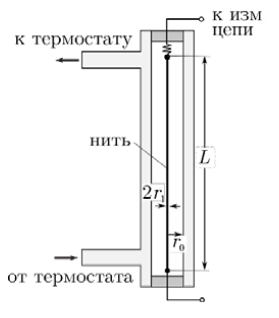
\includegraphics[width=1\textwidth]{scheme.png}
\end{minipage}


\newpage

Металлическая нить служит как источником тепла, так и датчиком температуры (термометром сопротивления). По пропускаемому через нить постоянному току I и напряжению U на ней вычисляется мощность нагрева по закону Джоуля–Ленца:

\begin{equation*}
	Q = UI,
\end{equation*}
и сопротивление по закону Ома:
\begin{equation*}
	R = \frac{U}{I}
\end{equation*}

Сопротивление нити является однозначной функцией её температуры R(t). Для большинства металлов относительное изменение сопротивления из-за нагрева невелико: приизменении температуры на 1 градус относительное изменение сопротивления нити может составлять приблизительно от 0,2 \%до 0,6\% (в зависимости от её материала).Следовательно, измерение R важно провести с высокой точностью.

\begin{center}
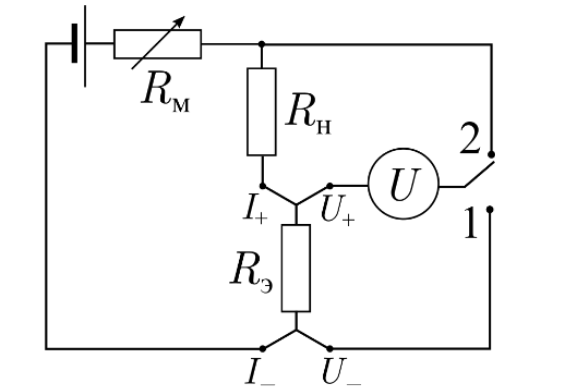
\includegraphics[width=0.7\textwidth]{elec.png}
\end{center}

Схема предусматривает использование одного вольтметра и эталонного сопротивления $R_э\sim10 \: Ом$, включённого последовательно с нитью. В положении переключателя 2 вольтметр измеряет напряжение на нити, а в положении 1 — напряжениена $R_э$, пропорциональное токучерез нить. Для исключения влияния контактов и подводящих проводов эталонное сопротивление $R_э$ также   необходимо подключать в цепь по четырёхпроводной схеме.
Ток в цепи в обеих схемах регулируется с помощью реостата или магазина сопротивлений $R_м$, включённого последовательно с источникомнапряжения.
\textbf{Методика  измерений.} В исследуемоминтервалетемператур (20–70 °C)зависимость сопротивле-ния  от температуры можно с хорошей точностью аппроксимировать линейной функцией:

\begin{equation*}
	R(t) = R_{273} \cdot (1+\alpha t)
\end{equation*}

где t — температурав [°C], $R_{273}$ — сопротивление нити при температуре 20C и $\alpha = \frac{1}{R_{273}} \frac{dR}{dT}$ — температурный коэффициент сопротивления материала.

\newpage

\textbf{Результаты обработки экспериментальных точек занесены в таблицу:}

\begin{table}[h!]
\begin{center}
\caption{$R_0$ и $\frac{dR}{dQ}$ для различных температур, $\kappa$}
\begin{tabular}{|c|c|c|c|c||c|c|c|}
\hline
T,C&$\frac{dR}{dQ},\frac{Ом}{мВт}$&$R_0$, Ом&$\sigma R_0$, \%&$\sigma \frac{dR}{dQ}, 10^{-5}$&$\frac{dQ}{d(\Delta T)}, \frac{Вт}{К} \cdot 10^{-2}$&$\kappa$, $\frac{Вт}{К\cdotм}\cdot 10^{-3}$&$\sigma \kappa$\\
\hline
60&0.00998&152.5&3&5&1.59&33&0.09\\
\hline
55&0.00999&153.2&3&6&1.59&33&0.09\\
\hline
50&0.00990&154.3&5&8&1.61&34&0.12\\
\hline
45&0.00974&155.5&2&4&1.63&34&0.09\\
\hline
40&0.00829&155.3&6&10&1.92&40&0.13\\
\hline
70&0.00837&157.4&7&8&1.90&40&0.13\\
\hline
\end{tabular}
\end{center}
\end{table}

\large{\textbf{Построим график зависимости $R_0$ от T:}}

\begin{equation*}
\end{equation*}

\begin{tikzpicture}[scale=1.7]
	\begin{axis}[
		axis lines = left,
    	xlabel = {T, C},
    	ylabel = {\textit{R}, Ом},
    	ylabel style={red, scale=0.7},
    	xlabel style={red, scale=0.7},
    	xmin=35, xmax=75
		]
		\addplot +[blue, only marks,
		] plot[
			error bars/.cd,
			y dir=both,
			y explicit relative,
			x dir=both,
			x fixed=0.1,
		] table [		    	    	    	
			x=A, 
			y=B,
			y error=err,
		]{exitMain};
		\addplot[color=red, domain=35:70]{146.234 + 0.159 * x};

	\end{axis}
\end{tikzpicture}

\begin{equation*}
\end{equation*}

Из графика определим угловой коэффициент $\frac{dR}{dT} = (0.159 \pm 0.014)$ Ом/К и $\alpha = \frac{1}{R_{273}} \frac{dR}{dT} = (1.06 \pm 0.10) \cdot 10^{-3}$ 1/К.
Занесем данные значений $\frac{dQ}{d(\Delta T)}$ в Таблицу 1.

\newpage

\large{\textbf{Построим графики зависимости $\kappa$ от T и ln($\kappa$) от ln(T):}}

\begin{equation*}
\end{equation*}

\begin{minipage}{.5\textwidth}
\begin{tikzpicture}[scale=0.8]
	\begin{axis}[
		axis lines = left,
    	xlabel = {T, C},
    	ylabel = {$\kappa$, Вт/(К$\cdot$м)$\cdot 10^{-3}$},
    	ylabel style={red, scale=0.7},
    	xlabel style={red, scale=0.7},
    	xmin=35, xmax=75
		]
		\addplot +[blue, only marks,
		] plot[
			error bars/.cd,
			y dir=both,
			y explicit relative,
			x dir=both,
			x fixed=0.1,
		] table [		    	    	    	
			x=A, 
			y=B,
			y error=err,
		]{exitKappa};

	\end{axis}
\end{tikzpicture}
\end{minipage}
\begin{minipage}{.5\textwidth}
\begin{tikzpicture}[scale=0.8]
	\begin{axis}[
		axis lines = left,
    	xlabel = {ln(T)},
    	ylabel = {ln($\kappa$)},
    	ylabel style={red, scale=0.7},
    	xlabel style={red, scale=0.7},
    	xmin=5.74, xmax=5.80,
		]
		\addplot +[blue, only marks,
		] plot[
			error bars/.cd,
			y dir=both,
			y explicit,
		] table [		    	    	    	
			x=A, 
			y=B,
			y error=err,
		]{exitln};
		\addplot[color=red, domain=5.74:5.80]{-7.80 + 0.764 * (x)};
		

	\end{axis}
\end{tikzpicture}
\end{minipage}

\begin{equation*}
\end{equation*}

(При построении ln($\kappa$) от ln(T) и последующих вычислениях не были учтены последние две экспериментальные точки, так как они явно не вписываются в зависимость и являются выбросами)

Из второго графика получим $\beta = (0.8\pm0.3)$. Что не согласуется с предсказаниями теории, утверждающие $\beta = \frac{1}{2}$

\textbf{Вывод:} Данный метод подходит для вычисления \textit{коэффициента теплопроводности} воздуха, но его точности недостаточно для достоверного определения зависимости последнего от \textit{температуры}.






















\newpage


\textbf{Относительная погрешность:} 0.0035\% + 0.0005\%$\cdot\frac{U_{диап}}{U_{изм}}$ для всех измерений

\begin{equation*}
\end{equation*}

\begin{minipage}{.3\textwidth}
\begin{center}
\begin{tabular}{|c|c|}
\hline
T = 40С&\\
\hline
$U_{R_0}, мВ$ \linebreak &$U_{R_0}$, \linebreak В\\
\hline
225.0&3.450\\
\hline
200.0&3.063\\
\hline
150.0&2.293\\
\hline
125.0&1.910\\
\hline
100.0&1.527\\
\hline
75.00&1.145\\
\hline
50.00&0.763\\
\hline
	\end{tabular}
	\end{center}
\end{minipage}% This must go next to `\end{minipage}`
\begin{minipage}{.3\textwidth}
\begin{center}
\begin{tabular}{|c|c|}
\hline
T = 45C&\\
\hline
$U_{R_0}, мВ$&$U_{R_0}$, \linebreak В \\
\hline
225.0&3.465\\
\hline
200.0&3.077\\
\hline
150.0&2.303\\
\hline
125.0&1.918\\
\hline
100.0&1.534\\
\hline
75.00&1.150\\
\hline
50.00&0.766\\
\hline
\end{tabular}
\end{center}

\end{minipage}
\begin{minipage}{.3\textwidth}
	\begin{center}
	\begin{tabular}{|c|c|}
	\hline
	T = 50C&\\
	\hline
	$U_{R_0}, мВ$&$U_{R_0}$, \linebreak В \\
	\hline
225.0&3.502\\
\hline
200.0&3.111\\
\hline
150.0&2.329\\
\hline
125.0&1.939\\
\hline
100.0&1.551\\
\hline
75.00&1.157\\
\hline
50.00&0.770\\
\hline
	\end{tabular}
	\end{center}

\end{minipage}

\begin{equation*}
\end{equation*}

\begin{minipage}{.3\textwidth}

	\begin{center}
	\begin{tabular}{|c|c|}
	\hline
	T = 55C&\\
	\hline
	$U_{R_0}$, мВ&$U_{R_0}$, \linebreak В \\
	\hline
225.0&3.517\\
\hline
200.0&3.123\\
\hline
150.0&2.338\\
\hline
125.0&1.947\\
\hline
100.0&1.557\\
\hline
75.00&1.167\\
\hline
50.00&0.778\\
\hline
	\end{tabular}
	\end{center}
\end{minipage}
\begin{minipage}{.3\textwidth}

	\begin{center}
	\begin{tabular}{|c|c|}
	\hline
	T = 60C&\\
	\hline
	$U_{R_0}$, мВ&$U_{R_0}$, \linebreak В \\
	\hline
225.0&3.508\\
\hline
200.0&3.115\\
\hline
150.0&2.332\\
\hline
125.0&1.942\\
\hline
100.0&1.554\\
\hline
75.00&1.165\\
\hline
50.00&0.776\\
\hline
	\end{tabular}
	\end{center}
\end{minipage}
\begin{minipage}{.3\textwidth}

	\begin{center}
	\begin{tabular}{|c|c|}
	\hline
	T = 70C&\\
	\hline
	$U_{R_0}$, мВ&$U_{R_0}$, \linebreak В \\
\hline
200.0&3.159\\
\hline
150.0&2.366\\
\hline
125.0&1.971\\
\hline
100.0&1.576\\
\hline
75.00&1.181\\
\hline
50.00&0.787\\
\hline
	\end{tabular}
	\end{center}
\end{minipage}

\begin{equation*}
\end{equation*}




\begin{minipage}{.3\textwidth}

\begin{tikzpicture}[scale=0.6]
	\begin{axis}[
		axis lines = left,
    	xlabel = {Q, Вт},
    	ylabel = {\textit{R}, Ом},
    	ylabel style={red, scale=0.7},
    	xlabel style={red, scale=0.7},
    	xmin=0, xmax=9,
    	title={40C},
		]
		\addplot +[blue, only marks,
		] plot[
			error bars/.cd,
			y dir=both,
			y explicit relative,
		] table [		    	    	    	
			x=B, 
			y=A,
			y error=err,
		]{exit40};
		\addplot[color=red, domain=0:9]{152.547 + 10 * 0.009982 * x};

	\end{axis}
\end{tikzpicture}
\end{minipage}
\begin{minipage}{.3\textwidth}

\begin{tikzpicture}[scale=0.6]
	\begin{axis}[
		axis lines = left,
    	xlabel = {Q, Вт},
    	ylabel = {\textit{R}, Ом},
    	ylabel style={red, scale=0.7},
    	xlabel style={red, scale=0.7},
    	xmin=0, xmax=9,
    	title={45C},
		]
		\addplot +[blue, only marks,
		] plot[
			error bars/.cd,
			y dir=both,
			y explicit relative,
		] table [		    	    	    	
			x=B, 
			y=A,
			y error=err,
		]{exit45};
		\addplot[color=red, domain=0:9]{153.2200 + 10 * 0.009993 * x};

	\end{axis}
\end{tikzpicture}
\end{minipage}
\begin{minipage}{.3\textwidth}

\begin{tikzpicture}[scale=0.6]
	\begin{axis}[
		axis lines = left,
    	xlabel = {Q, Вт},
    	ylabel = {\textit{R}, Ом},
    	ylabel style={red, scale=0.7},
    	xlabel style={red, scale=0.7},
    	xmin=0, xmax=9,
    	title={50C},
		]
		\addplot +[blue, only marks,
		] plot[
			error bars/.cd,
			y dir=both,
			y explicit relative,
		] table [		    	    	    	
			x=B, 
			y=A,
			y error=err,
		]{exit50};
		\addplot[color=red, domain=0:9]{154.923 + 10 * 0.009900 * x};

	\end{axis}
\end{tikzpicture}
\end{minipage}

\begin{minipage}{.3\textwidth}

\begin{tikzpicture}[scale=0.6]
	\begin{axis}[
		axis lines = left,
    	xlabel = {Q, Вт},
    	ylabel = {\textit{R}, Ом},
    	ylabel style={red, scale=0.7},
    	xlabel style={red, scale=0.7},
    	xmin=0, xmax=9,
    	title={55C},
		]
		\addplot +[blue, only marks,
		] plot[
			error bars/.cd,
			y dir=both,
			y explicit relative,
		] table [		    	    	    	
			x=B, 
			y=A,
			y error=err,
		]{exit55};
		\addplot[color=red, domain=0:9]{155.536 + 10 * 0.009740 * x};

	\end{axis}
\end{tikzpicture}
\end{minipage}
\begin{minipage}{.3\textwidth}

\begin{tikzpicture}[scale=0.6]
	\begin{axis}[
		axis lines = left,
    	xlabel = {Q, Вт},
    	ylabel = {\textit{R}, Ом},
    	ylabel style={red, scale=0.7},
    	xlabel style={red, scale=0.7},
    	xmin=0, xmax=9,
    	title={60C},
		]
		\addplot +[blue, only marks,
		] plot[
			error bars/.cd,
			y dir=both,
			y explicit relative,
		] table [		    	    	    	
			x=B, 
			y=A,
			y error=err,
		]{exit60};
		\addplot[color=red, domain=0:9]{155.238 + 10 * 0.008291 * x};

	\end{axis}
\end{tikzpicture}
\end{minipage}
\begin{minipage}{.3\textwidth}

\begin{tikzpicture}[scale=0.6]
	\begin{axis}[
		axis lines = left,
    	xlabel = {Q, Вт},
    	ylabel = {\textit{R}, Ом},
    	ylabel style={red, scale=0.7},
    	xlabel style={red, scale=0.7},
    	xmin=0, xmax=9,
    	title={70C},
		]
		\addplot +[blue, only marks,
		] plot[
			error bars/.cd,
			y dir=both,
			y explicit relative,
		] table [		    	    	    	
			x=B, 
			y=A,
			y error=err,
		]{exit70};
		\addplot[color=red, domain=0:9]{157.436 + 10 * 0.008377 * x};


	\end{axis}
\end{tikzpicture}
\end{minipage}









\end{document}


\lipsum[1-4]
\begin{wrapfigure}{R}{5cm}
	\centering
	\includegraphics[width=0.20\textwidth]{rd.png}
	\caption{1}
\end{wrapfigure}
\lipsum[1-6]


\begin{figure}[h]
\begin{center}$
\begin{array}{cccc}
	\includegraphics[width=0.20\textwidth]{rd.png}&
	\includegraphics[width=0.20\textwidth]{rd.png}&
	\includegraphics[width=0.20\textwidth]{rd.png}&
	\includegraphics[width=0.20\textwidth]{rd.png}\\
	(1) & (2) & (3) & (4)
\end{array}$
\end{center}
\end{figure}

